\documentclass[11pt]{article}
\usepackage{fullpage,amsthm,amsfonts,amssymb,epsfig,amsmath,times,amsthm}
\usepackage{algpseudocode}
\usepackage{tikz}
\usepackage[boxruled,vlined,linesnumbered]{algorithm2e}
\usepackage{ulem}

\newtheorem{theorem}{Theorem}
\newtheorem{claim}[theorem]{Claim}

\theoremstyle{definition}
\newtheorem*{solution}{Solution}
\newtheorem*{algo}{Algorithm}
\newtheorem*{proofcorr}{Proof of correctness}
\newtheorem*{analysis}{Big-O Analysis}

\begin{document}
% PUT YOUR INFORMATION IN THESE TWO LINES 
\hfill Isai  Lopez Rodas  

\hfill 1605542  ilopezro@ucsc.edu

\begin{center}
{\bf\Large 
CMPS 102 --- Spring 2020 --  Homework 3 %Solutions (draft version)
}
\end{center}

\begin{center}
Five problems, due Friday May 1 (on canvas) and Monday May 11 (11:59 PM) on Gradescope.  \\
\textit{Due class size, it is likely that only a subset of the problems will be graded.} \\
Ver 0405.2
\end{center}

%\newcommand{\set}[1]{\{ #1 \}}
%\newcommand{\qed}{ \large \hfill $\Box$ \\ \medskip }
%\newcommand{\qedq}{ \large \hfill $\Box$?? \\ \medskip }

% \emph{This is the draft version of written homework two.  
% The questions will not change, but I am distributing it early so 
% you can start thinking about the problems and help catch any ambiguities 
% or typos before the final version of the homework is posted.  } 

\medskip

\renewcommand{\P}{\mbox{IH}}

\noindent
Before you begin the assignment, please read the following carefully.
\begin{itemize}
    \item\textbf{ Read the \emph{Homework Guidelines}}.
    \item Every part of each question begins on a new page. Do not change this.
    \item This does not mean that you should write a full page for every question. Your answers should be short and precise. Lengthy and wordy answers will lose points.
    \item Do not change the format of this document. Simply type your answers as directed.
    \item You are \textbf{not} allowed to work in teams.
\end{itemize}
%Complete the following.
\emph{I have read and agree to the collaboration policy.}  -- Isai Lopez Rodas, ilopezro@ucsc.edu
% replacing "FirstName LastName, email@ucsc.edu" with your information.
\\
Collaborators: None%write the name of the collaborators. If you worked by yourself, please write 'none'.
\\
\hrule
\begin{enumerate}

\item (1 pt) Take the pre-quiz on Canvas by 11 PM on Friday May 1st.  This will be short quiz designed to test
 if you have read and understood the other problems.  The quiz should be available by Thursday afternoon.


\item (6 pts):  Chapter 4, Problem 2. Two true or false statements, with justification (3 pts each).
\begin{solution}
Problem 2.
\begin{itemize}
    \item This would be \textbf{true} because Kruskal's Algorithm would sort them in the same exact way, but the subsets of the edges in the MST would be the same because this algorithm 
    only takes a look at the order of the costs rather than the actual given values. 
     \item This would be \textbf{false} because if we were given edges in a given graph with edges $(s,v)$, $(v,t)$, and $(s,t)$ with values 2, 5, and 6 then we know that $(s,t)$ is the shortest
	 path because it has value 6; however, if we were to square the values of each edge we would have the following values: $(s,v)$, $(v,t)$, and $(s,t)$ with values 4, 25, and 36. Now, the shortest path
	would be $(s,v)$ and $(v,t)$ with a value of 29. 
\end{itemize}
\end{solution}
\newpage
%Complete the following.
\emph{I have read and agree to the collaboration policy.}  -- Isai Lopez Rodas, ilopezro@ucsc.edu
% replacing "FirstName LastName, email@ucsc.edu" with your information.
\\
Collaborators: None%write the name of the collaborators. If you worked by yourself, please write 'none'.
\\
\hrule
\item (3 + 5 + 5 + 2 = 15 pts). 
The Menlo Park Surgical Hospital admitted a patient, Mr. Banks, who was in a car accident and is still in critical condition and needs continuous monitoring over the next 48 hours (i.e.~all real-valued times between 0 and 48).
At any given time only one nurse needs to be on call for the patient though. 
For this we have an availability interval for each of the $n$ nurses, 
which is a time from which they become available, $a_i$, to the time they must leave for other commitments, $b_i$
%(for $i$ from 1 to $n$).
The $a_i$ and $b_i$ are real valued, and you may assume that for each $i$, $0\leq a_i < b_i \leq 48$.
You need to devise an algorithm that determines a set of nurses to use to cover the next 48 hours of Mr. Banks' stay while having the minimum number of nurses disrupt their normal routine to be on call for him (or report that some time cannot be covered)
A nurse leaving at the same time as another arrives is acceptable. 
Following is a picture of what the intervals for the nurses might look like. 
The darker bars correspond to a set 
of 5 of the 10 nurses who can cover the entire duration. (Notice, though, that 4 nurses would have sufficed.)

\begin{center}
	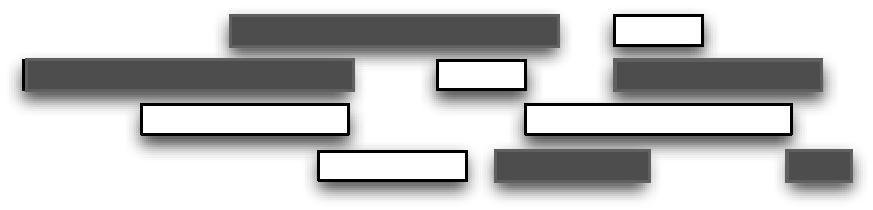
\includegraphics[height=1in]{subcover}
\end{center}

Your efficient {\bf greedy} algorithm should take as input a list of pairs of times $(a_i,b_i)$ for $i=1$ to $n$ and the end time $T$.

\textit{Continued on next page.}
\newpage
\begin{enumerate}
	\item Consider the greedy algorithm that selects nurses by
	repeatedly choosing the nurse who will be there for the longest
	time among the periods not covered by previously selected
	nurses. For example,if times 2 through 8 are covered by already selected nurses a another nurses interval is (5,10),
	then adding that nurse would only provide additional coverage form 8 to 10, or 2 units of time. 
	Give an example showing that this algorithm does \textbf{not}
	always find the smallest set of nurses.
	\begin{solution}
	\item This algorithm is not the most efficient because it does not choose the smallest set of available nurses. If we have three nurses with the following 
	schedules:
	\begin{itemize}
		\item Nurse 1: 0-24
		\item Nurse 2: 10-45
		\item Nurse 3: 24-48
	\end{itemize}
	The algorithm will choose nurse 2 first since it has the longest available schedule. Nurse 2 is able to cover 35 hours while nurse 1 and 2 can only cover 24 hours. 
	This is a problem because you need someone to cover the first 10 hours and the last 3 hours. Therefore the algorithm will \textbf{HAVE} to schedule nurses 1 and 2. Therefore
	the algorithm has chosen all three nurses when there is a more optimal solution, which is to choose nurses 1 and 3 to cover the shifts. Therefore, this algorithm is not correct. 
	\end{solution}
	\newpage
	\item Present an algorithm that always outputs a smallest subset of nurses that can cover the entire 48 hours 
	or report that no such subset exists.
	\begin{solution}
		\item 
		\begin{enumerate}
			\item For all $a_i$, sort in ascending order. 
			\begin{enumerate}
				\item If there are two nurses who have the same $a_i$, sort $b_i$ in decending order. 
			\end{enumerate}
			\item After this sorting is done, we not have a list of nurses and their schedules where nurse 1 is (ideally) supposed to start off at the 0$^{th}$ hour. 
			\item If $a_0 > 0$, there is no solution. 
			\item Else if $a_0 = 0$, then the first scheduled nurse is $(a_0, b_0)$
			\item Starting at $i=1$, look for a $a_i$ that fits the following inequality: $a_i \leq b_0$. Once you find a nurse that fits the following, you are 
			guaranteed to have a nurse$_1$ either start before or when nurse$_0$ ends. We will keep a counter for the index $x$ where $b_x$ is the biggest. 
			\begin{enumerate}
				\item If you've got a situation when $a_1 > b_0$, you have no solution because that means that no nurse is able to start when nurse$_0$'s shift ends. 
				\item After an iteration finds such an $a_i > b_1$, we set a variable $y = i$. 
			\end{enumerate}
			\item The next nurse that can cover the next shift then becomes: $(a_y, b_y)$
			\item Next loop would start at $i=y$. Line $v, v.A,$ and $v.B$ would be repeated as neccesary. 
			\item Iteration of this loop would end when $b_i$ = 48. 
		\end{enumerate}
	\end{solution}
	\newpage
	\item Prove that your algorithm is correct (i.e.\ alway finds a smallest possible subset of the nurses the cover the entire stay).
	\begin{solution}
	\item 
	We will begin with assuming we have a solution, $s_1$, produced by the algorithm above. 
	\\[1em]
	\textbf{\textit{Base Case:}} Another solution exists besides the one provided by $s_1$
	\\
	Therefore we know that $a_0 = 0$ is true because there must exist a nurse that covers that first hour. We also know that the $b_1 \geq b_i$. Therefor if we replace
	$(a_i, b_i)$ with $(a_1, b_1)$, we still have a valid solution, thus the greedy choice applies in this case. 
	\\[1em]
	\textbf{\textit{Inductive Step:}} Assume there is another different solution that starts with $(a_i, b_i)$. Therefore, we want to prove that:
	\begin{center}
		$a_i = a_0, b_i = b_0, a_{i+1} = a_y, b_{i+1}=b_y, \cdots, a_{i+j} = a_{y+j}, b_{i+j}=b_{y+j}$
	\end{center}
	where 
	\begin{center}
		$b_{y+j} > b_{y+j+1}$
	\end{center}
	To satisfy the fact that there must be a valid nurse that can start at the scheduled end time for the previous nurse. The greedy algorithm will find the a value for $b_{y+j}$ while 
	acknowledging inequality: $a_{i+j} \leq b_{i+y+1}$. Therefore we can replace $(a_i, b_i)$ with $(a_{i+j}, b_{i+j})$. Which procudes a valid solution according to the greedy choice application.
	Therefore, the algorithm is correct. 
	\end{solution}
	\newpage
	\item State its running time with a brief one-to-three sentence justification. 
	\begin{solution}
	Because we are sorting the nurses at the beginning of the algorithm, the sorting takes $\mathcal{O}(n\log n)$ time. The comparisons in the middle are only made once 
	per element, which then produces an $\mathcal{O}(n)$ runningtime for the comparisons. Therefore, the total runningtime of the algorithm is $\mathcal{O}(n\log n)$. 
	\end{solution}
	\newpage
\end{enumerate}
%Complete the following.
\emph{I have read and agree to the collaboration policy.}  -- Isai Lopez Rodas, ilopezro@ucsc.edu
% replacing "FirstName LastName, email@ucsc.edu" with your information.
\\
Collaborators: None %write the name of the collaborators. If you worked by yourself, please write 'none'.
\\
\hrule
\item (15 pts) A first grade teacher has a set of $n$ books, say $\{1, 2, \ldots, n\}$, stored on a bookshelf in the classroom.
Each book $k$ has a popularity represented by the probability $p(k)$ of being wanted by a student (since these are probabilities they are non-negative and sum to 1). 
Unfortunately, the students are not sophisticated enough to do binary search, and so do a sequential search 
for the book from left to right.   When $s_1$ is the first book on shelf, $s_2$ the second, and so on, 
and some book $s_i$ is wanted, it will time $i$ for the student to locate it. 
When all the books are on the shelf, the average search time is $\sum_{i=1}^n i \cdot p(s_i)$.  
The problem is to find (and prove correct) a greedy algorithm that that takes the $p(k)$ values and 
determines an order $s_1, s_2, \ldots , s_n$ for storing the books on the shelf that minimizes this average search time.

(Hint: Use the structure of the problem or an exchange argument to prove your greedy algorithm's solution is optimal.)

\textit{Continued on next page.}
\newpage
%Answer beings on a new page.
\begin{algo}


\end{algo}
\newpage
\begin{proofcorr}

\end{proofcorr}
\newpage
\begin{analysis}

\end{analysis}
\newpage

%Complete the following.
\emph{I have read and agree to the collaboration policy.}  -- Isai Lopez, ilopezro@ucsc.edu
% replacing "FirstName LastName, email@ucsc.edu" with your information.
\\
Collaborators: None %write the name of the collaborators. If you worked by yourself, please write 'none'.
\\
\hrule
\item (15 pts)  Is it a break-in?

The security staff for a high-tech company suspects that a notorious hacker is breaking into their network and stealing their trade secrets.   
The traffic on the network over the last couple of days is represented by a sequence of 
events $E=(e_1, e_2, \ldots, e_n)$
where each $e_i$ is an integer event ID.  
These IDs can come from all sorts of applications, and the same event number can be seen multiple times.
The notorious hacker has a predictable way to break in:  he causes a particular 
sequence of $k<n$ events $H=(h_1, h_2, \ldots, h_k)$ to happen on the network to help him gain access.
These events have to occur in that particular order, and some event numbers may be be repeated in $H$.
Your task is to design and prove correct a greedy algorithm for determining if $H$ is a subsequence of $E$
\uline{and when the hacker could have broken in.}
Recall that $H$ is a subsequence of $E$ if $H$ is embedded in $E$, i.e.~some number (possibly 0) of the events in $E$ can be deleted so that your are left with $H$.  
More formally, the $k$ length sequence $H$ is a subsequence of $E$ if there is a sequence of $k$ indices 
$i_1 < i_2 < \cdots < i_k$ such that each $h_j = e_{i_j}$.

For example, neither (2, 4, 5) nor (4, 2, 2, 5) are subsequences of 
(1, 9, 4, 1, 4, 2, 6, 5, 7), but (9,5) and (4, 4, 2, 5) are.

\uline{
Design a greedy algorithm running in $O(n)$ time that determines if $H$ is a subsequence of $E$ and returns
the first (lowest) $\ell$ such that $H$ is a substring of $E_\ell = e_1, e_2, \ldots, e_\ell$ 
(i.e.~$E_{\ell}$ is the shortest prefix of $E$ that contains $H$ as a substring).
Prove that your algorithm is correct and briefly justify its running time.
}

\uline{
To prove correctness, it may be helpful for your algorithm to compute the sequence of indices where
the events in $E$ match those in $H$.
}

\textit{Continued on next page.}
\newpage
%Answer beings on a new page.
\begin{algo}
	\item
	\begin{algorithmic}[1]
		\Procedure{isBreakIn}{$E, H$}
		\State $lenE \leftarrow len(E)$
		\State $lenH \leftarrow len(H)$
		\State $counter \leftarrow 0$
		\State for (i = 0); i$<$lenE and counter $<$ lenH; i++
		\State if(E[i] = H[counter]) 
		\State counter++;
		\State if (counter = i )
		\State return i
		\State return -1
		\EndProcedure
	\end{algorithmic}
\end{algo}
\newpage
\begin{proofcorr}
	\item
When we have a sequence of evenets $E_1$ that is also in $H$ the algorithm selects the first event in $E_1$ that matches with $E_1$. It will 
then proceed to that with subevent $e_2 \cdots e_i$. After, our algorithm will return the index in which $E$ is a subsequence of $H$. Therefore, 
our algorithm's greedy choice is the optimal solution. 
\end{proofcorr}
\newpage
\begin{analysis}
In the worst case scenario, our algorithm will have to go through all events in $E$, which means that it has to run a total time of $\mathcal{O}(n)$.
\end{analysis}
\newpage

\end{enumerate} 
\end{document}
